% IEEEAerospace2012.cls requires the following packages: times, rawfonts, oldfont, geometry
\documentclass[twocolumn,letterpaper]{IEEEAerospaceCLS}  % only supports two-column, letterpaper format

% The next line gives some packages you may find useful for your paper--these are not required though.
%\usepackage[]{graphicx,float,latexsym,amssymb,amsfonts,amsmath,amstext,times,psfig}
\usepackage[]{graphicx,float,latexsym,amssymb,amsfonts,amsmath,amstext,times}
% NOTE: The .cls file is now compatible with amsmath!!!

\usepackage[ampersand]{easylist}
\usepackage[]{graphicx}    % We use this package in this document
\usepackage{url}
\usepackage{todonotes}
\newcommand{\ignore}[1]{}  % {} empty inside = %% comment

\begin{document}
\title{Planetary Rover Simulation for Lunar Exploration Missions}

\author{%
}

\maketitle

\thispagestyle{plain}
\pagestyle{plain}

\maketitle

\thispagestyle{plain}
\pagestyle{plain}

\begin{abstract}

When planning planetary rover missions it is useful to develop intuition and skills driving in, quite literally, alien environments before incurring the cost of reaching said locales. Simulators make it possible to operate in environments that have the physical characteristics of target locations without the expense and overhead of extensive physical tests. To that end, NASA Ames and Open Robotics collaborated on a lunar rover driving simulator based on the open source Gazebo simulation platform and leveraging ROS (Robotic Operating System) components. The simulator was integrated with research and mission software for rover driving, system monitoring, and science instrument simulation to constitute an end-to-end lunar mission simulation capability.

Although we expect our simulator to be applicable to arbitrary lunar regions, we designed to a reference mission of prospecting in polar regions. The harsh lighting and low illumination angles at the lunar poles combine with the unique reflectance properties of lunar regolith to present a challenging visual environment for both human and computer perception. Our simulator placed an emphasis on high fidelity visual simulation in order to produce synthetic imagery suitable for evaluating human rover drivers with navigation tasks, as well as providing test data for computer vision software development.

In this paper, we describe the software used to construct the simulated lunar environment and the components of the driving simulation. Our synthetic terrain generation software artificially increases the resolution of lunar digital elevation maps by fractal synthesis and inserts craters and rocks based on lunar size-frequency distribution models. We describe the necessary enhancements to import large scale, high resolution terrains into Gazebo, as well as our approach to modeling the visual environment of the lunar surface. An overview of the mission software system is provided, along with how ROS was used to emulate flight software components that had not been developed yet.

We summarize how the simulator has been used to refine the mission concept of operations and to evaluate the operations impact of rover engineering design decisions. We reduced uncertainty about mission operations tempo by simulating mission scenarios with representative drive speeds, telemetry rates and network delays. The operations team exploited the simulator’s flexibility to experiment with different rover configurations and compare the effect of things such as different camera placement options and mobility system steering constraints.

Finally, we discuss the effect of using the high-fidelity synthetic lunar images for visual odometry.  We also discuss the characterization of the shader model for lunar illumination relative to a ray-tracing with accurate reflectance models.  Further, we characterize the wheel slip model, and find some inconsistencies in the produced wheel slip behaviour.

\end{abstract}


\tableofcontents

%%%%%%%%%%%%%%%%%%%%%%%%%%%%%%%%%%%%%%
\section{Rough Outline (feel free to change)}
%%%%%%%%%%%%%%%%%%%%%%%%%%%%%%%%%%%%%%
\begin{easylist}[checklist]
& Resource Prospector Background
&& High level overview of mission objectives (Fong/Deans)
&& Differences to Mars ops (Furlong/Deans)
&& High level concept of operations (Deans/Shirley/Allan/Furlong)
&& High level software architecture (Furlong/Allan)
&&& flight/ground software split (Furlong)
& Simulator goals / overview 
  && Development approach
    &&& create driving sim as fast as possible
    &&& development/refinement of conops
  && prototype mission software architecture with stubs and existing components with ROS (Gerkey)
  && use sim-generated data for flight software development
      &&& flight software --> Gazebo
      &&& Gazebo and ROS output --> nav and localization
    && incrementally replace stubs and emulated components with flight versions
    && use for training
& Synthetic Terrain Generation (Allan/Wong)
& Lunar Visual Environment (Allan/Wong)
  && Gazebo terrain enhancements (Chen)
    &&& LOD
    &&& background tiles (Allan)
  && GLSL shader (Allan/Wong/Welsh)
  && Wheel tracks
  && Shadows (Welsh/Chen)
    &&& real time shadow challenges 
    &&& baked shadows (Shirley)
    &&& Gazebo shadow improvements 
  && Ephemeris (McMichael)
  && Lighting / HDR
    &&& Earthshine, bounced light (Wong)
    &&& high bit depth rendering in Gazebo (Chen)
    &&& PBR indirect lighting experiment (Wong)
    &&& attempt to reproduce in GLSL (Allan)
& Vehicle simulation 
  && Use existing, similar robots to emulate (Furlong)
    &&& Husky
    &&& KRex2
  && Flight software integration with Gazebo
  && Wheel slip plugin (Rogg/Peters)
    &&& first order approximation
    &&& fault injection
& Flight Software Prototype (Furlong)
  && flight/ground split
  && emulation with ROS components
  && Ops software
    &&& WARP
    &&& VERVE
  && Science sim and software
& Driving ConOps Experiments (Deans)
& Results
  && stereo visual odometry (Welsh)
  && lunar illumination comparison (Wong)
  && wheel slip results (Allan/Rogg/Peters)
 \end{easylist} 


%%%%%%%%%%%%%%%%%%%%%%%%%%%%%%%%%%%%%%
\section{Introduction}
%%%%%%%%%%%%%%%%%%%%%%%%%%%%%%%%%%%%%%



Lunar polar environment different to prior extra-terrestrial rover missions. Mars has long time delays that make interactive commanding impossible, lunar comm delays enable semi-interactive commanding. Science involved in operations. Operations needed to develop and mature concept of operations.  

\section{Background}


Lunar surface operations provide for qualitatively different mission operation scenarios than what is possible in the Martian surface.  The most important aspect is the broad swings in temperature on the Moon.  From lunar day to lunar night there can be swings in temperature of over three hundred degrees.  Building a robot to survive lunar night comes with additional costs and reliance on heat sources, like the radioactive materials used in the Lunokhod missions \cite{XXX}.  This can increase mission complexity substantially.  

If the rover is not designed to survive lunar night then the mission either has the time pressure to complete in fourteen days, or the operational pressure to chase sunlight to peaks of eternal light, as proposed in \cite{otten2018strategic}.  The Resource Prospector mission planned to operate within the constraints of the lunar solar day, creating a need for high-tempo mission operations. 

Lunar regolith presents two challenges, both relating to the microbombardment processes which produce the soil \cite{XXX}.  Because the lunar soil is not produced by the erosion processes we are accustomed to on Earth the particular matter is sharp, which is a hazard to the vehicle, and it has reflectance properties very much unlike the Earth\todo{cite Hapke models}, which poses a challenge to both human and automated perception systems. \todo{I think this is too much information about regolith up front. Especially since we have to explain how we implement the reflective properties in the shader below. -uland}

The Moon is not without its operational advantages.  First, the relative closeness of the Moon means that the time-of-flight communications delay is only 2.5 seconds, and not on the order of minutes\todo[author=pmf]{get time of flight delay for Mars} for a Mars mission.  Second, through the use of the Deep Space Network, it is possible to be in constant communication with a lunar surface vehicle, barring shadows from terrain features.  Constant availability of a rover supports the high-tempo mission cadence missions like Resource Prospector.


Taking advantage of the high communications availability we designed our autonomy system to be distributed between the rover on the surface of the moon and the remote operations team on Earth.  The architecture would place lower-level components of an autonomous system -- e.g., waypoint following, relative pose estimation, vehicle safeguarding \todo{Is safeguarding the word we use?} -- on-board the robot.  Higher-level algorithms 


\section{Simulator Approach}

Early in mission development, there are many unknowns. As the various mission elements work to address their specific requirements within budget and technology constraints, the trade space is large and a design decision in one element may have ripple effects that impact overall system performance. One way to reduce uncertainty about design alternatives and to answer questions about system performance, particularly from an operational perspective, is through simulation. For example, it may be obvious that a skid steer mobility system would be simple, cheap, and robust from a mechanical perspective but odometry from an explicit steer platform would give superior localization results. But how would the driving behavior of those platforms impact solar charging rates over a traverse? 

Our goal was to create a simulation environment in which we could rapidly create approximate prototypes of lunar rover systems to estimate characteristics and performance. Due to the broad scope of the simulation and the desire to have a functional, end-to-end lunar driving simulation as quickly as possible, a simulation framework that offered a rich set of off-the-shelf capability was necessary. [ why ROS and Gazebo were a great choice - *Gerkey* ] 


\section{Synthetic Terrain Generation}

To produce a viable lunar driving experience the simulated world must be representative of the target physical environment. Specifically, the morphology of the terrain should accurately represent terrain features that would be considered either positive or negative obstacles for the rover. Although DEMs are available for much of the lunar surface, the resolution of these models are not sufficient to represent rover-scale hazards. To make matters worse, the best resolution lunar DEMs are generated from stereo orbital imagery, yet the reference mission was targeting areas with permanently shadowed regions. 

On the Moon, the principal obstacles of interest to rovers are rocks and craters. Getting the "density" right was one of the primary objectives of this work as the distributions of obstacles have significant impact on mission traverse paths and schedule. While mean values are published in literature [cite JPL report 1969] for Highlands/Mare/Polar regions, these size-frequency distributions vary widely according to locality. Parameters such as proximity to large or fresh craters, in particular, are significant modulating factors for rocks. We attempted to model these variations by procedural placement of craters and ejecta fields and simulating the processes of Lunar terrain formation with the most current orbital information. 

In our process, crater distributions are first sampled to produce an estimate of size-frequency per unit area. For a scene of specific dimension, we can predict how many craters of a particular diameter are present. These distributions take an inverse-exponential form introduced in [jpl report 1969]. We have updated parameters for Polar regions based on manual identification in LRO images and curve fitting. Variation from uncertainty is allowed by estimating sigma from fitting residuals. In the case where the scene is based on a prior DEM, large craters are identified by hand and this is factored into the sampled distribution so that double counting does not occur. Next, an age is assigned pseudo-randomly to each crater, with the probability of a crater being old decreasing with size such that small craters are uniform. The sampled distribution is ordered sequentially in time and assigned a flag based on whether it is large enough to generate ejecta. Working forward in time, ejecta generating craters are "placed" by assigning a uniform random (x,y) location while their shape is stencilled onto a spatial probability map used to generate ejecta rocks. Shape consists of an interior, rim, and ejecta blanket which are all tunable physical parameters. Small craters do not generate ejecta and are thus only assigned spatial coordinates without contributing to the ejecta map.           

Unlike craters, it is difficult and time consuming to identify existing rocks from orbital imagery for each terrain. Moreover, small rocks are under image resolution limits and must be extrapolated from models. Thus, all rocks are generated by randomly sampling from distributions of size-frequency similar to craters. There are two populations associated with rocks, one for ejecta thrown during crater formation, and a second uniform background distribution for terrain between large craters. For the Polar regions, the background distribution is several orders of magnitude sparser than ejecta. During the process of sampling rocks and assigning spatial coordinates, the ejecta probability map is consulted in order to modulate local density. At each time step, old rocks have a probability of being covered by regolith, and a new crater forming will cover old rocks under its extent. When the number of generated rocks and craters equals the expected number plus some variation, the sizes, ages, and coordinates of the features are passed into fractal terrain generator.     

Because the reference mission defined rocks larger than 10-25cm as positive obstacles, we desired a terrain resolution of 5cm or greater. Given that 5cm resolution is well beyond available lunar DEMs, we developed tools to artificially increase resolution using established techniques {parkes2004planet}. ** insert summary of PANGU paper **

The diamond-and-square method of fractal terrain generation is straightforward to implement and a reasonable choice for adding higher frequency details. However, the method is known to create interpolation artifacts when constrained {miller1986definition}, particularly on low frequency features like aged crater rims. We employed two approaches to mitigate these artifacts. First, we replace linear interpolation with Catmull-Rom splines in the diamond-and-square algorithm which reduces the severity of the artifacts. Second, prior to scaling up we split the terrain into high and low frequency components by running a low pass filter on the DEM, and subtracting it from the original. The high frequency component is scaled up with the diamond-and-square algorithm whereas the low frequency component is scaled up with bilinear interpolation. Craters are inserted into the low frequency component before adding the high and low frequency components back together to reconstitute the DEM. This process is repeated until the desired resolution is reached. 

In addition to the enhanced GeoTIFF DEM, the synthetic terrain generation process produces other assets that will be used for appearance modeling in Gazebo. An albedo map is generated by inserting crater splash patterns using crater location, size, and freshness parameters. The excavated regolith from a fresh crater impact is lighter in shade due to lack of exposure to solar radiation, and over time the ejecta blanket weathers and blends into the surrounding terrain. An exponential function applied to the freshness parameter determines ejecta ray lightness. Next, a rock mask maps which cells in the DEM correspond to regolith and which cells correspond to rocks. Finally, we generate a normal map which captures the surface normal at each DEM posting. 



\section{Lunar Visual Environment}
some text

\subsection{Gazebo Terrain Improvements}

As high resolution synthetic terrains are generated and used in simulation, it became evident that the existing terrain visualization support in Gazebo has its performance limitations. At the highest resolution of 8K in our experiments, the DEM can take up to several minutes to load in Gazebo, and once loaded, a significant drop in framerate was observed. To address these performance issues, we added two features to Gazebo: 1) caching of terrain data to disk, and 2) Level-Of-Detail (LOD) support. Gazebo uses the Ogre3D rendering engine, which conveniently has support for both of these features. 

\subsubsection{Terrain data caching}

It was observed that a large portion of the Gazebo startup time was attributed to the loading and parsing of DEM data into Ogre3d internal terrain tile data format. Adding the ability to cache these data means that the overhead would only need to be incurred once. All subsequent Gazebo sessions using the same DEM file and textures will fetch and load the generated Ogre3D terrain cache from disk, bypassing the DEM parsing and terrain tile generation process. In our tests, the Gazebo startup time reduced by a factor of 10 (from ~5 minutes to ~30 seconds) when loading a simulation environment constructed from an 8K resolution DEM.

\subsubsection{LOD}

The most noticeable drop in runtime rendering performance occurs when the entire terrain is within the camera view, in which case, no parts of the terrain are frustum-culled. While the camera sensors onboard on rover do not necessary see the entire terrain, the degraded performance was affecting normal usage of the simulator such as basic user interaction with the simulation environment. Integrating LOD support helped to reduce the triangle count and hence improves the frame rate in this scenario (see figure \ref{fig:heightmaplod}). The quad-tree based LOD implementation in Ogre3D lets users configure LOD transitions to some degree by specifying the maximum screen pixel error allowed when rendering. In general, a node higher up the tree, i.e. lower detail, can only be rendered if its screen space pixel error, computed based on the height characteristics of the node and the current camera distance, does not exceed the specified maximum. 

\begin{figure}[h!]
	\includegraphics[width=\columnwidth]{figures/heightmap_lod_bright.jpg}
   	\caption{Wireframe visualization of terrain with LOD enabled}
    \label{fig:heightmaplod}
\end{figure}

Enabling LOD helped resolved framerate issue but in some cases, especially when large DEMs are used, it introduced noticeable popping effects during LOD transitions. This issue was mitigated by pre-subdividing the DEM into smaller terrain chunks. In doing so, we also had to make sure that the UV coordinates of each terrain chunk are transformed so that the texture maps, which applies to the whole terrain, can be sampled correctly during shading.

\subsubsection{Terrain Meshes}

[*Allan* to describe terrain dae meshes?]

\subsection{GLSL Shader}
Regolith is the layer of powdery dust which covers most of the moon except for the rare vertical rocky surface. As such, correctly simulating the appearance of regolith via the bidirectional reflectance distribution function (BRDF) is a major factor in achieving visual fidelity. The reflectance of Lunar regolith and regolith-like materials have been comprehensively studied and the Hapke functions remain the most accurate physically-based models \cite{hapke11}. However, the Hapke BRDF has several drawbacks when used for rover-scale rendering including mathematical complexity, non-invertibility, and edge artifacts\cite{wong2012}. We implement an approximation to the full BRDF suggested by Hapke, which combines coherent-backscatter and shadow hiding into a single term. Furthermore, our Hapke approximation shader is combined with a Lambertian BRDF with a nadir-dependent angle to reduce rendering artifacts. This is a similar strategy used by \cite{McEwen1996} in developing the Lunar-Lambertian model derived from Lommel-Seeliger reflectance. Our Hapke parameters are estimated from prior literature for Highlands regolith, which is a stand-in for Polar regions of the moon. Our model achieves the desired loss of contrast and opposition surge while behaving properly under direct illumination.           

\subsection{Shadows}
Shadow rendering provides countless challenges and has been under continuous development since the advent of computer graphics. Like most aspects of real-time computer graphics, a good solution involves finding a set of approximations that work well for you particular problem. Our problem was to render shadows that would appear as realistic as possible from the perspective of our rover's cameras. And, since one of our simulation goals was exploration of polar regions, we needed a shadow solution that would support low illumination angles (i.e. the sun close to the horizon).

For our purposes, we were only concerned with shadows cast by the sun. On a rover, any lights would necessarily be mounted close to the rover's cameras, so the shadows they cast would be mostly hidden from view.

The dominant real-time shadow technique and the one we used is called shadow mapping. It involves rendering a texture map that contains the depth of objects in a scene from the point-of-view of a light source and then comparing these depths with object positions when rendering the scene from the user's point-of-view. These comparisons reveal which surfaces are illuminated by the light and which are in shadow. There are other shadow techniques, but shadow mapping provides a popular combination of speed and flexibility.

\subsubsection{Real-time Shadow Challenges}
One common challenge related to shadow mapping is providing an appropriate amount of shadow map resolution in every part of a scene. Ideally, shadow detail decreases with distance from the user's point of view such that there is a unique shadow map texel for every pixel in the final image. In a small scene (e.g. indoors) a uniform distribution of shadow resolution can work well enough. However, when rendering a landscape out to the horizon, a uniform distribution of shadow resolution is impractical from the standpoint of memory consumption.

A related challenge stems from the relationship of the light ray direction compared to the user's view direction. When these directions are close to parallel, as is often the case in our simulation because the sun is close to the horizon, it becomes difficult to make a good distribution of shadow resolution. This is known as the dueling frusta problem. There are refinements of shadow mapping that exaggerate this problem and others that minimize it.

It is possible to improve shadow quality if you know, for a given scene, which shadows are static and which are dynamic. If the light source moves then all the shadows it casts are dynamic. The orientation of the sun relative to the moon changes so slowly that we can assume it is effectively stationary in our simulation. The only moving object is the rover itself. Therefore, we can pre-compute shadows cast by the terrain (often referred to as baked shadows), and we only need to compute real-time shadows for the rover.

\subsubsection{Baked Shadows}

Because the sun moves slowly (~0.5 deg/hour), we elected to pre-render the shadows generated by the terrain shadowing itself, capturing the result in a lightmap that was used by the shader to render static shadows with very little runtime overhead.

To generate the lightmap, a 2-dimensional form of ray-tracing called ray-casting was used because the terrain was modeled as a height field with no overhangs.  (Our approach is very similar to the technique used in Wolfenstein 3D on the PC.)  The lightmap was calculated at the same 4 cm resolution as the terrain, and the sun was modeled as an extended source with rays cast from 280 points within the sun's disk.

This approach produces high-quality shadows over the whole terrain, with smoothly varying penumbras cast by distant features and tiny shadows cast by one pixel bumps.  For any given rover camera image, most of these shadows are too distant to see; the most important shadows are close to the rover, particularly those cast by the rover itself and rendered using the real-time techniques described above.  But the static shadows are very visible in the gazebo camera used for debugging and their soft edges add to the images' realism.

While the sun moves slowly, it's not fixed.  The sun's disk is also 0.5 deg, so any terrain pixel can potentially go from fully lit to fully unlit or vice versa within one hour.  This only happens at the edges of shadows, however, and is rarely important to rover operations because the rover's path is planned to avoid these areas.  Our approach to this slow movement is to linearly interpolate between two lightmaps in the shader, however, this enhancement has not been implemented yet.

\subsubsection{Gazebo Shadow Improvements}
Gazebo originally used a shadow mapping technique called Parallel Split Shadow Maps (PSSM) to render real-time shadows. On the surface, this was a good choice because PSSM uses multiple shadow maps to provide a quality distribution of shadow resolution, even in the dueling frusta case. However, there were several problems with the implementation that conspired to ruin the shadows in our simulation, often leaving us with low-resolution shadows or no shadow on parts of the screen.

Gazebo uses Ogre3D for rendering, and so it was using Ogre3D's PSSM implementation for rendering shadows. Each shadow map in that implementation was also being processed by a Light-Space Perspective Shadow Map (LiSPSM) technique, which performs poorly in the dueling frusta case and also exhibited some mysterious bugs. Additionally, Ogre3D assumes all scenes are oriented with the y-axis pointing up while gazebo assumes the z-axis points up. This decreased the usable region of each shadow map and often caused shadow edges to be more jagged than necessary. We corrected both problems by adding code to Gazebo that bypasses these troublesome parts of Ogre3D.

To further refine the PSSM implementation, we added hooks to the Gazebo API that allow aspects of the shadows to be tuned through Gazebo plugins. We were then able to affect the relative size of the shadow maps and the distance from the observer within which shadows would be applied.

With the resolution distribution problems mitigated, we turned to the overall lack of shadow resolution. The easiest first step was to increase Gazebo's default shadow map resolution from 1024 to 2048. This double our resolution everywhere, but there were still small features on the rover, such as the mast, that were not casting shadows consistently. The shader that Gazebo was using to apply shadows was smoothing shadow edges using Percentage Closest Filtering (PCF) with a 3x3 grid of sample positions. This worked well for smoothing jagged shadow edges, but, due to the filter's uniformity, sometimes small features would fall through the cracks and not affect the final shadow intensity. We replaced PCF with something known as hardware PCF, a common graphics driver hack that accomplishes the same type of smoothing with little performance impact. Then we applied a 9-sample Poisson filter (not a uniform grid like before), which smoothed the shadows even more and does a much better job of preserving small features.

\subsection{Wheel Tracks}
Any rover will leave wheel tracks in the powdery lunar regolith. We wanted to include these tracks in our visual simulation for realism and as an orientation aid for operators. It would be possible to reshape the terrain geometry to represent wheel tracks, but this method is difficult to implement and would provide more fidelity than we needed. A much simpler alternative is to use a technique called bump mapping to give the illusion of wheel tracks on flat geometry.

Our shader already employs bump mapping to give the regolith its fine detail, so we expand on this to add wheel tracks. We apply a 1-channel texture to the drivable area of the terrain. It starts out with every texel set to the maximum value, 255. Wherever a rover wheel travels we draw a groove in the texture, setting texels to 0 or some medium value. Wherever this texture is less than 255, the shader mixes a surface normal into the bump mapping. To approximate a surface normal it compares neighboring texels in the wheel tracks texture to find the slope in the x- and y-directions. Assuming a z-value of 1.0, the three values are normalized to produce a final surface normal.

To draw the wheel tracks in the texture we use a Gazebo plugin. We use Gazebo's knowledge of the rover model and the terrain layout to compute what part of the texture each wheel position corresponds with. Everywhere each wheel travels, we draw an anti-aliased dot in the texture of a size in texels that appears to match the wheel size when the texture is projected on the terrain. These dots overlap to give the appearance of a continuous groove made by each wheel.

\subsection{Ephemeris}

The position of the Sun and Earth relative to the moon is computed using the SPICE C toolkit provided by the Navigation and Ancillary Information Facility (NAIF) \url{https://naif.jpl.nasa.gov/naif/toolkit.html}.  Using the timestamp maintained by the simulator, this toolkit generates the transformations between the Moon, the Sun, and the Earth at the current simulated time.  By chaining these transformations with the rover's current position on the surface of the moon we are able to compute the positions of the Sun and the Earth relative to our local coordinate system and position them accurately in the simulator.  We are not concerned about the locations of stars because they are not drawn in the simulator.

\subsection {Photometry}
The reference mission required training in use of photographic systems coupled with active illumination for driving. Developments were made to model complex illumination effects from natural sources, rover-based lighting, and finally sensor processes in order to produce an accurate camera image. To accomplish this in a real-time manner, we used physically-based raytracing to produce exemplar scenes which were then approximated with shader tricks. 

The dynamic range of scenes on the Moon drives the performance of stereo safeguarding, human situational awareness, and the design of rover lighting. To accurately simulate dynamic range, global illumination must be modeled. If direct sunlight were the only source of illumination, shadows would be pitch black. However, we know this is not the case in images of the Lunar surface despite the high dynamic range. Light reaches shadowed areas from multiple natural sources including diffuse interreflection of the Lunar surface, Earthshine, and starlight. Using ray tracing, we simulated the contribution of indirect scattering in ideal surface craters given particular phase angle combinations. Our findings indicate that an average of 6\% of the direct illumination reflects into shadows in polar scenes. This effect was approximated in rendering by illuminating the scene with a low-intensity virtual source opposing the sun in azimuth \todo{is this true for the final version? -uland}. Analytically we also showed that light from the star field is insignificant and that Earthshine, while fractionally powerful compared to indirect scattering, is complexly dependent on the phase of Earth. Thus, these other sources were not implemented.       

lens flares\\
rover lights\\
16bit rendering image post processing\\



\section{Vehicle Simulation}


\subsection{Wheel Slip}
\textit{DRAFT ARNO}

The wheel/terrain interaction plays an important role in the fidelity of the simulation. In the real world, an input drive command will result in a non-zero slip of the rover wheel on loose terrain which will generate drift in localization algorithms. In order for this drift to be plausible in simulation, a wheel slip plug-in was developed and implemented for Gazebo based on a test results from two tests: RP single wheel drawbar pull test and RP lunar mass equivalent unit test (see figure \ref{fig:mgru}) in the SLOPElab facility at NASA Glenn Research Center (GRC) (ref: \url{https://www.nasa.gov/centers/glenn/events/tour_erb_slope.html}). The simulant for these test was GRC-1 (ref: \url{https://etd.ohiolink.edu/!etd.send_file?accession=case1269272964&disposition=inline}), which has similar mechanical characteristics as the lunar regolith. 
\begin{figure}[h!]
	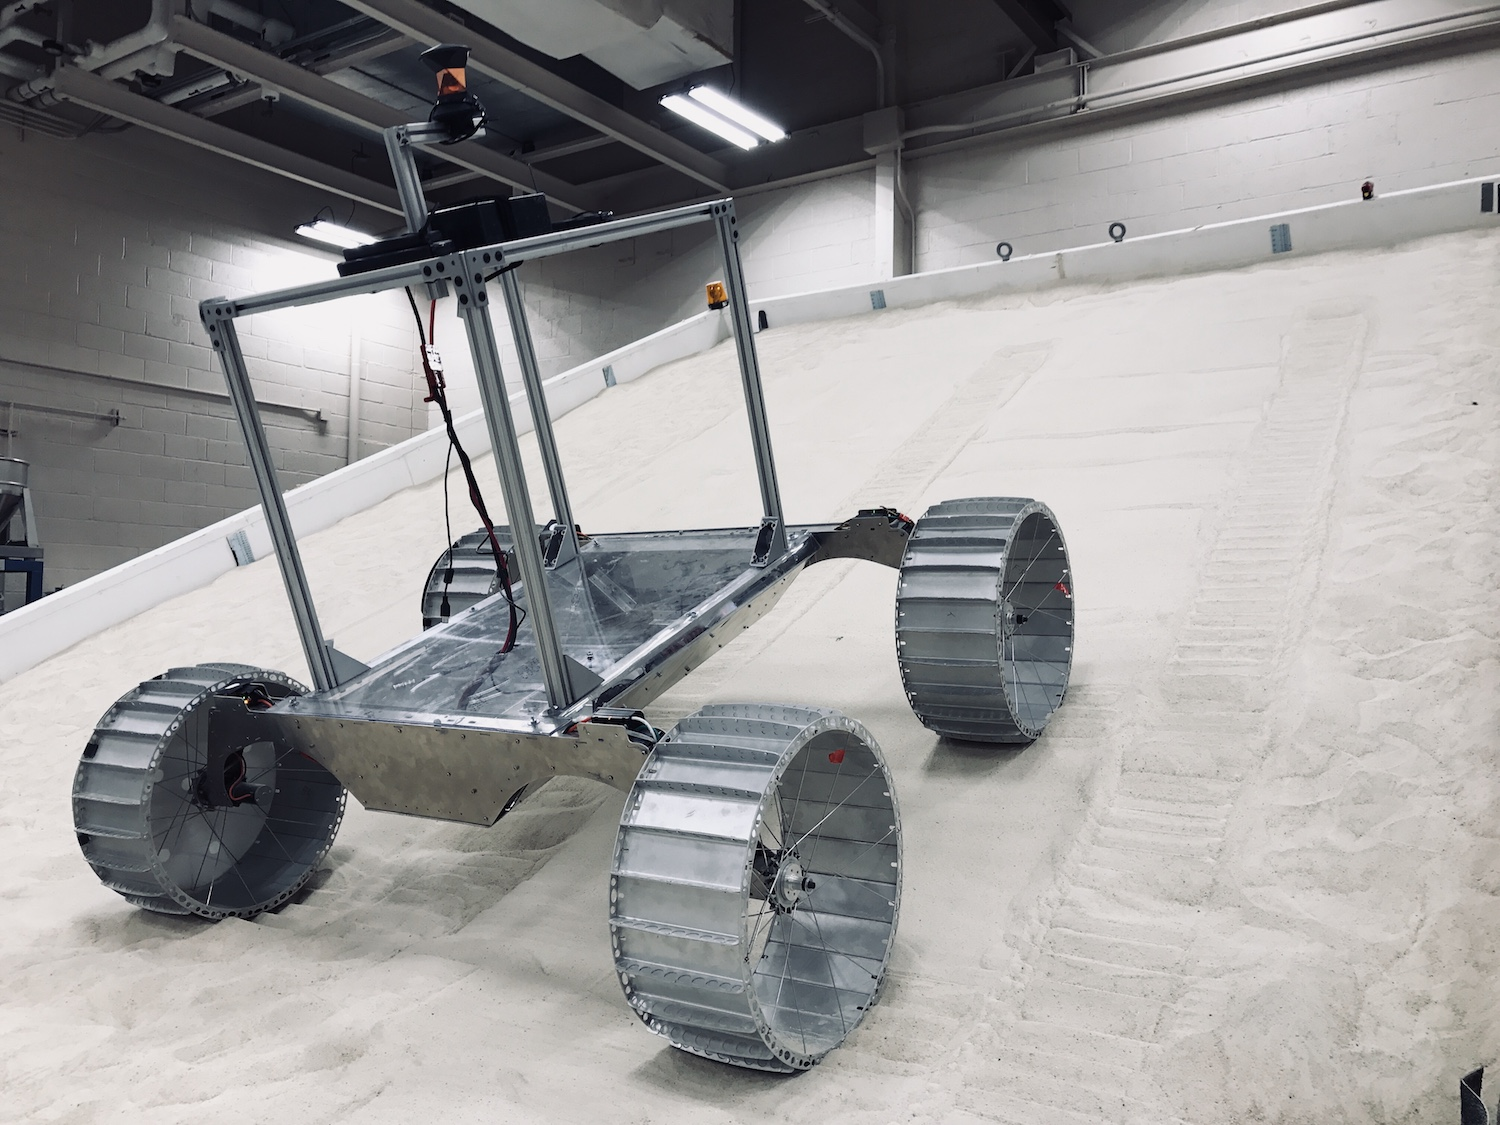
\includegraphics[width=\columnwidth]{figures/wheel_slip_MGRU.JPG}
   	\caption{A picture of the RP lunar mass equivalent rover at the SLOPElab in NASA GRC.}
    \label{fig:mgru}
\end{figure}
The Gazebo simulator physics engine provide the following framework to deal with wheel/terrain interaction (see figure \ref{fig:wheelsoilmodel}). The is based on the Coulomb-Mohr friction theory. With a compliance tuning parameter that enables to simulate loose material generating slip greater than zero on shallow angle slopes.
\begin{figure}[h!]
	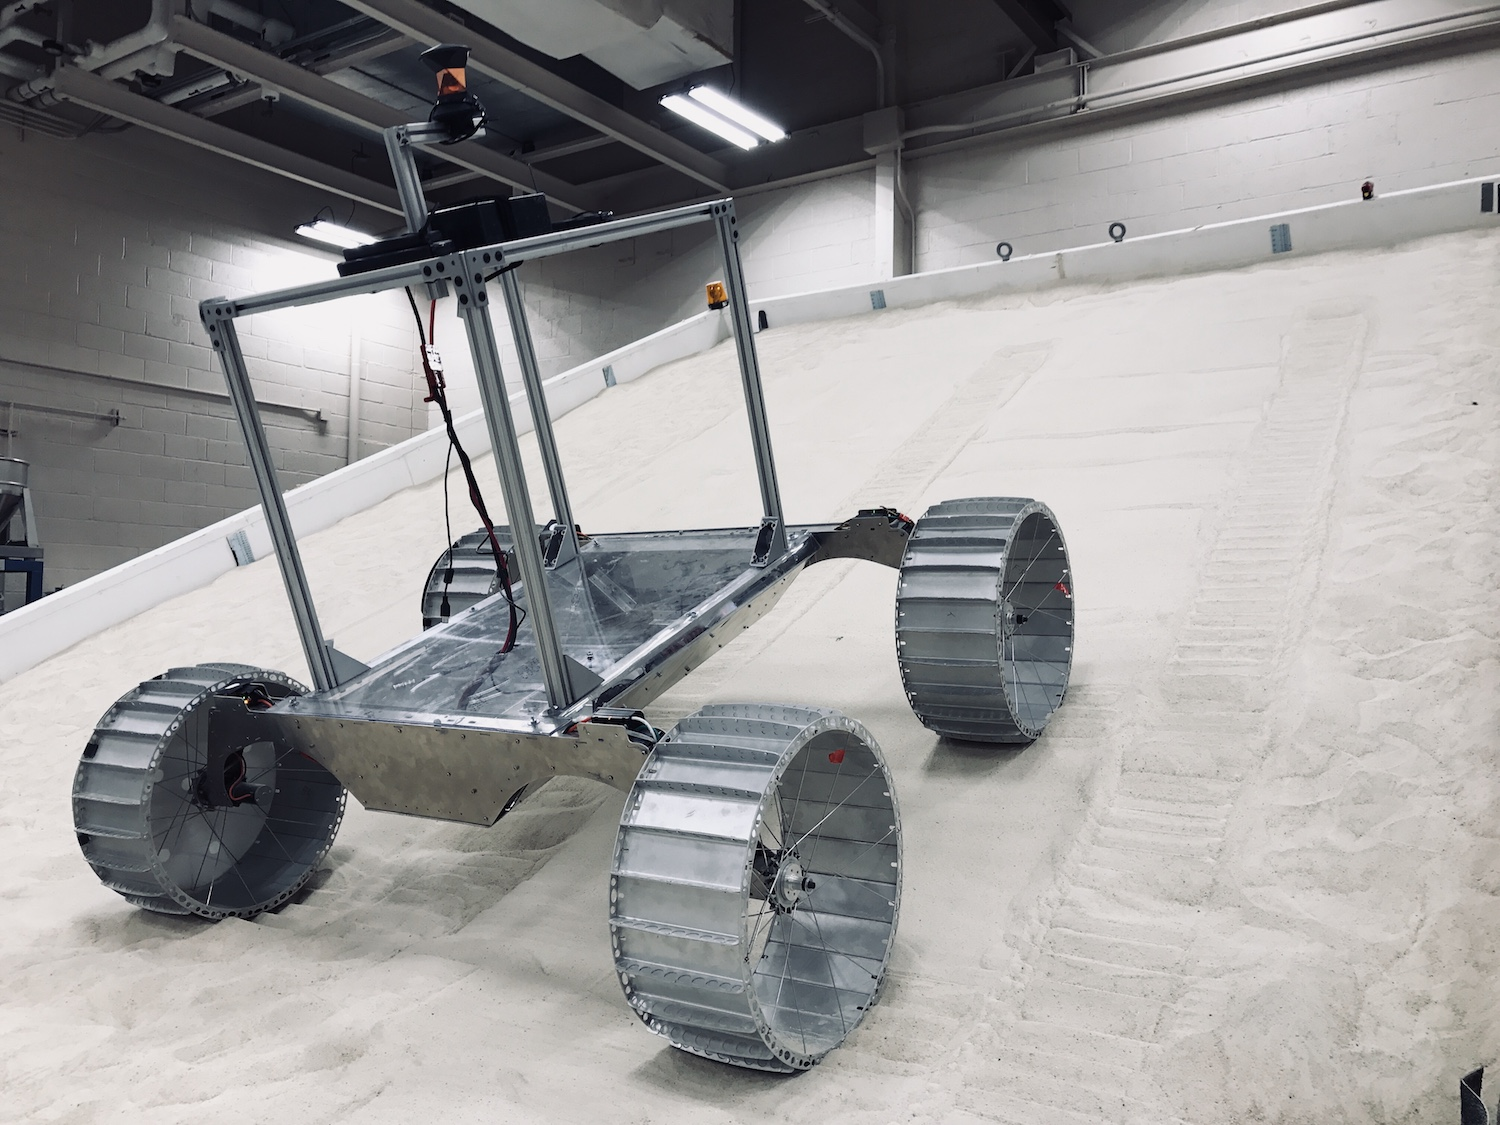
\includegraphics[width=\columnwidth]{figures/wheel_slip_MGRU.JPG}
   	\caption{Wheel/soil interaction model}
    \label{fig:wheelsoilmodel}
\end{figure}

Although not perfect at simulating the wheel/soil interaction, this plug-in enables the simulated rover to have a high level slip behavior relatively close to what will be expected on a lunar terrain. In order to increase the fidelity and give more realism for wheel sinkage and rover embedding, this simple model would need to be replaced by a discrete element method (DEM) model which is very costly in terms of computational power and existing system are unproven due to the complexity of the particle interaction.

\textit{END OF DRAFT ARNO}


\section{Results}

\subsection{Stereo Visual Odometry}
One of the goals of the visual simulation was to provide data for computer vision work, and an example of such work is the stereo visual odometry we implemented for Resource Prospector's ground software. It generates 3D point clouds from successive stereo camera images, aligns them using the Point Cloud Library's implementation of the Iterative Closest Point algorithm, and uses the transforms between point clouds to track changes in the rover's movements. This stereo visual odometry interacts with other software and sensors to estimate the rover's absolute pose.

To refine the mission's concept of operations, we wanted to know how much overlap is required between camera images for stereo visual odometry to be effective. The easiest way to lose overlap between successive images is by yawing the camera or rover, so that is the first test we ran. We learned that with camera rotations of 50-degrees or less, stereo visual odometry yields more accurate results than the wheel odometry we had been using (shown in the following graph).
\begin{figure}[h!]
	\includegraphics[width=\columnwidth]{figures/rotating_clouds_with_odom_error.png}
    \caption{TBD}
\end{figure}

We also learned that there are occasionally incorrect point cloud alignments, telling us we need to improve our alignment algorithm or find a way to detect the quality of each alignment. It is important to note the results we found for stereo visual odometry are preliminary. There are further tests to run and improvements to be made to both our visual simulation and visual odometry. For example, after a specific camera is chosen for the mission we will be able to refine our camera simulation. This will affect point cloud generation and require us to run these tests again.

\subsection{Wheel Slip}
In order to characterize the \texttt{wheel\_slip\_plugin}, we set up a test harness to gather data on wheel slip behavior over multiple runs. We created a Gazebo world with ramps from 0 to 30 degrees at 2 degree increments (see figure \ref{fig:simulationramps}). A rostest script would spawn the rover at the base of each ramp and command it to drive 10 meters forward. Wheel slip was measured by comparing dead reckoning distance driven to ground truth and test runs covered sets of parameter values for longitudinal compliance, physics engine solver iterations, and drive speed. 
\begin{figure}[h!]
	\includegraphics[width=\columnwidth]{figures/world_lots_o_ramps.jpg}
   	\caption{Gazebo simulation for the slip vs slope test with the RP rover.}
    \label{fig:simulationramps}
\end{figure}
Overall, the \texttt{wheel\_slip\_plugin} demonstrated the expected behavior and compared favorably with physical testbed results as can be seen in figure \ref{fig:wheelsliptuningchart}, which compares wheel slip measured from MGRU with the  \texttt{wheel\_slip\_plugin}. 
\begin{figure}[h!]
	\includegraphics[width=\columnwidth]{figures/wheel_slip_roverslip.png}
   	\caption{Comparison of the RP lunar mass equivalent rover slip on GRC-1 simulant and RP rover slip in the Gazebo simulator.}
    \label{fig:wheelsliptuningchart}
\end{figure}

However, our test results show that at certain angles and compliance values, there is a wide variation in measured wheel slip (see figure \ref{fig:slipdisparities}). Those disparities are particularly large on a flat terrain.
\begin{figure}[h!]
	\includegraphics[width=\columnwidth]{figures/slip_compliance_longitudinal.png}
   	\caption{Graph of the slip of the RP rover in Gazebo showing the disparities in the amount of slip.}
    \label{fig:slipdisparities}
\end{figure}

\textit{END OF DRAFT ARNO}








\end{document}
